\documentclass[dvipdfmx]{jarticle}
\usepackage{graphicx}
\usepackage[top=30truemm,bottom=30truemm,left=25truemm,right=25truemm]{geometry}
\usepackage{listings,jvlisting}

\lstset{
  basicstyle={\ttfamily},
  identifierstyle={\small},
  commentstyle={\smallitshape},
  keywordstyle={\small\bfseries},
  ndkeywordstyle={\small},
  stringstyle={\small\ttfamily},
  frame={tb},
  breaklines=true,
  columns=[l]{fullflexible},
  numbers=left,
  xrightmargin=0zw,
  xleftmargin=3zw,
  numberstyle={\scriptsize},
  stepnumber=1,
  numbersep=1zw,
  lineskip=-0.5ex
}

\begin{document}
\begin{titlepage}
    \begin{center}
        {\huge 情報科学演習C 課題1レポ―ト}
        \vspace{180pt}\\
        \begin{tabular}{rl}
            氏名 & 山久保孝亮\\
            所属 & 大阪大学基礎工学部情報科学科ソフトウェア科学コース\\
            メールアドレス & u327468b@ecs.osaka-u.ac.jp\\
            学籍番号 & 09B22084\\
            提出日 & \today\\
            担当教員 & 
        \end{tabular}
    \end{center}
\end{titlepage}
\section{課題1-1}
\begin{enumerate}
    \item ping exp001を実行すると以下の図1のような出力結果が得られる.
    \begin{figure}[h]
        \centering
        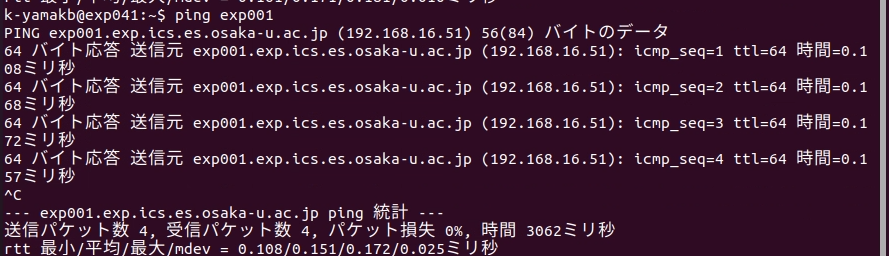
\includegraphics[width=8cm]{1-1-1.png}
        \caption{ping exp001の実行結果}
    \end{figure}
    \\pingコマンドはECHO\_REQUESTを使用してホストからECHO\_RESPONSEを引き出し、通信の状態を確認するコマンドである.ECHO\_REQUESTとECHO\_RESPONSEはICMPのメッセージである.
    1行目には第一引数で指定したホスト名(IPアドレス)と送信するパケットデータのサイズを表示している.2行目以降は同じ結果が繰り返し出力されている.
    繰り返されているそれぞれの内容は以下の通りである.
    \begin{itemize}
        \item 64バイト応答:送信されたデータサイズ
        \item 送信元:第一引数で指定したホスト名とIPアドレス
        \item icmp\_seq:pingを送信した回数
        \item ttl:パケットが破棄されるまでの期間の値
        \item 時間:パケットを送信して返信が来るまでの時間
    \end{itemize}
    そしてCtrl+Cを押して強制終了すると統計値が表示される.統計値の内容はパケット数を送信,受信した解すと損失した回数,pingコマンドを入力して終了するまでの時間,応答時間の最小値,平均値,最大値,標準偏差である.
    \item どちらのurlを入力した際でも同じ大阪大学のウェブサイトが開いた.このことから,www.osaka-u.ac.jpというドメインはIPアドレスに変換すると133.1.138.1となったと考えられる.
    \item nslookup osaka-u.ac.jpを実行すると以下の図2のような実行結果が得られる.
    \begin{figure}[h]
        \centering
        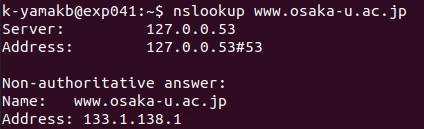
\includegraphics[width=8cm]{1-1-3.png}
        \caption{コマンドの実行結果}
    \end{figure}
    \\nslookupコマンドは二つのモードがあり,対話モードでは様々なホストやドメインに関する情報をネームサーバーに問い合わせたり、 ドメイン内のホストの一覧を表示したりすることができる.
    非対話モードではホストやドメインの名前と要求された情報だけを表示する.これによりドメイン名からIPアドレスを,IPアドレスからドメイン名を知ることができる.
\end{enumerate}
\section{課題1-2}
\begin{enumerate}
    \setcounter{enumi}{3}
    \item /usr/sbin/arp -aを実行すると以下の図3のような出力が得られる.
    \begin{figure}[h]
        \centering
        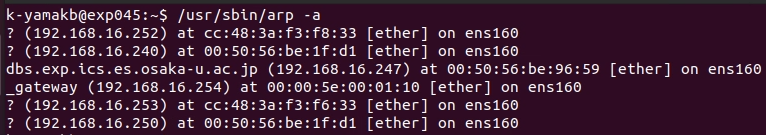
\includegraphics[width=8cm]{1-2-4.png}
        \caption{コマンドの実行結果}
    \end{figure}
    \\このコマンドによってARPキャッシュが出力として表示される.具体的な表示内容としては,まず最初にドメイン(IPアドレス)が表示され,その後atに続いてそれに対応するMACアドレスが表示される.
    [ether]というのはARPがIPアドレスをMACアドレスに変換する際にイーサネットフレーム内で動作するため表示されている.ens160というのはLinuxシステム上で特定のネットワークインターフェースを識別するための名前である.
    \item pingをexp002とexp003に対して実行すると以下の図4のような出力が得られた.
    \begin{figure}[h]
        \centering
        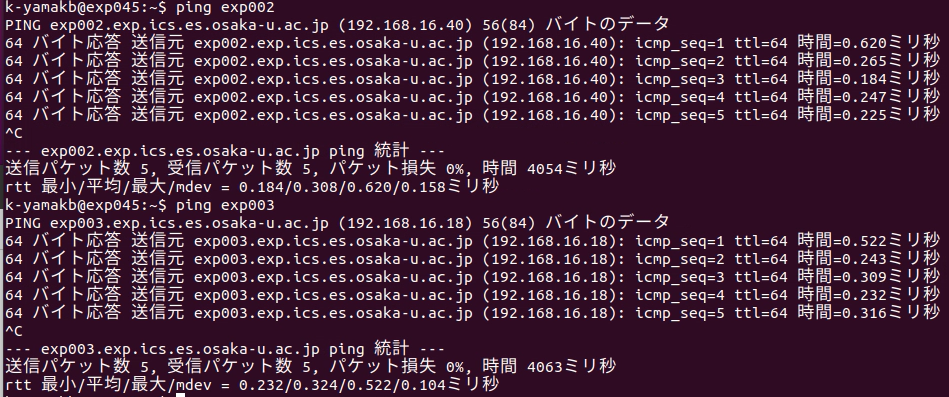
\includegraphics[width=8cm]{1-2-5.png}
        \caption{コマンドの実行結果}
    \end{figure}
    基本的な出力内容は課題1-1の1で述べた内容と同じであった.ただ,IPアドレスが異なっていた.
    \\以下の図5は図4の出力の後に/usr/sbin/arp -aを実行したときの出力である.
    \begin{figure}[h]
        \centering
        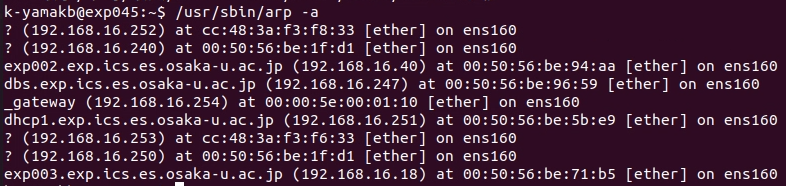
\includegraphics[width=8cm]{1-2-5-2.png}
        \caption{コマンドの実行結果}
    \end{figure}
    図3の出力結果と比べて,exp002とexp003のIPアドレスとMACアドレスのキャッシュが出力に追加されている.出力が変化した理由としては,pingコマンドによりメッセージのやり取りが行われたことで
    ARPキャッシュの内容が変化したためであると考えられる.
    \item /usr/sbin/tracerouteをexp002exp003,Webサーバ,ゲートウェイに対して実行すると以下の図6のような出力が得られる.
    \begin{figure}[h]
        \centering
        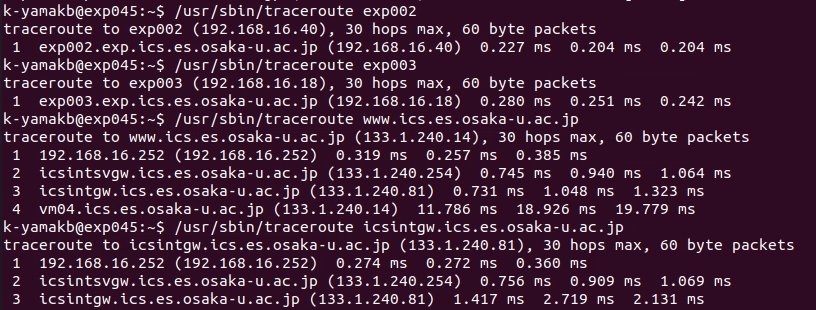
\includegraphics[width=8cm]{1-2-6.png}
        \caption{コマンドの実行結果}
    \end{figure}
    \\図6の出力結果を比較すると,exp002とexp003に対してtracerouteを実行したときは同じとなるがその二つとWebサーバ,ゲートウェイに対してtracerouteを
    実行したときには異なる結果となることがわかる.tracerouteコマンドは目的のIPアドレスまでの経路を表示するコマンドであり,それぞれ目的地のIPアドレスが異なるために
    出力の内容が異なると考えられる.
    \item pingが正しく動作することでそのIPアドレスがネットワーク内にあると推測することができる.また,exp002とexp003に対してtracerouteを実行した際に経路がexp002しか出力されなかったことから,デバイスとしてexp002やexp003が存在することが考えられる.
    Webサーバに対してtracerouteを実行した際に,まず実際のIPアドレスである192.168.16.252を通りその後仮想IPアドレスである192.168.16.254を通ってからWebのドメインを通っていたことから,ホストはまずデフォルトゲートウェイに接続されてその後仮想アドレスが割り当てられたデバイスに接続される.
    \item /bin/netstat -rを実行すると以下の図7のような実行結果が得られる.
    \begin{figure}[h]
        \centering
        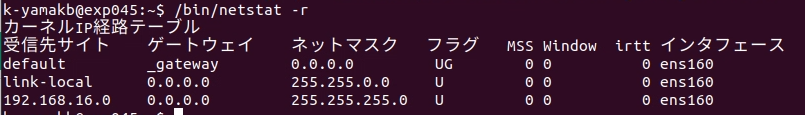
\includegraphics[width=8cm]{1-2-8.png}
        \caption{コマンドの実行結果}
    \end{figure}
    netstatはrオプションで実行するとネットワークの経路を出力する.具体的な出力内容は以下のようになる.
    \begin{itemize}
        \item 受信先サイト:送信されたパケットの宛先ネットワークまたはIPアドレス.
        \item ゲートウェイ:パケットが送信される際に使用されるゲートウェイのIPアドレス.
        \item ネットマスク:ネットワークプレフィックスの長さを示すサブネットマスク.
        \item フラグ:ルーティングエントリの状態や特性を示すフラグ.
        \item MSS:通信に使用されるTCPセグメントの最大サイズ.
        \item Window:TCPウィンドウサイズ.
        \item irtt:通信の初回往復時間.
        \item インターフェース:ルートで使用されているネットワークインターフェースを示す.
    \end{itemize}
    このことから,自分が想像したネットワークは
    \item 
\end{enumerate}
\section{課題1-3}
\begin{enumerate}
\setcounter{enumi}{9}
    \item C言語の標準ライブラリ関数とは
    \item ac
\end{enumerate}
\section{発展課題}
\section{感想}
\section{謝辞}
\section{参考文献}
\end{document}